\documentclass[10pt,a4paper]{amsart}
\usepackage[margin=19mm]{geometry}
\usepackage{amsmath,amssymb,mathtools}
\usepackage[scr=rsfs,cal=euler]{mathalfa}
\usepackage{xfrac}
\usepackage[unicode,hidelinks,bookmarks=false]{hyperref}
\newcommand{\ie}{i.e.\ }
\newcommand{\cf}{cf.\ }
\newcommand{\resp}{respectively\ }
\newcommand{\Subsection}{\subsection}
\providecommand{\nobreakdash}{\nobreak\hbox{-}}
\setlength{\emergencystretch}{2em}
\multlinegap0pt
\usepackage{tikz}
\usepackage{xfrac}
\usepackage{amssymb}
\usepackage{xcolor}
\usepackage{float}
\newtheorem{lemma}{Lemma}
\newcommand{\David}[1]{\textcolor{red}{[David] #1}}
\newcommand{\M}{\mathcal{M}}
\newcommand{\N}{\mathbb{N}}
\newcommand{\ceil}[1]{\left\lceil #1 \right\rceil}
\newcommand{\chris}[1]{\textcolor{purple}{[Chris] #1}}
\newcommand{\floor}[1]{\left\lfloor #1 \right\rfloor}
\title{$C$-complexes, Clasp Number, and Triple Linking Number}
\author{Christopher William Davis, David Lawrence, Jack Paulsen, Nathan Phillips}
\date{Source: arXiv:2607.22848v1 (CC BY 4.0)}
\begin{document}
\maketitle

\noindent\emph{Source and licence.} $C$-complexes, Clasp Number, and Triple Linking Number. Version arXiv:2607.22848v1 (CC BY 4.0), distributed by arXiv under the Creative Commons Attribution 4.0 International licence, http://creativecommons.org/licenses/by/4.0/, as recorded in the arXiv licence metadata for this exact version and shown on the abstract page https://arxiv.org/abs/2607.22848v1. Full licence notice: \texttt{licenses/arxiv-2607.22848-CC-BY-4.0.txt}.\par\smallskip

\noindent\textit{Editorial scope.} Counted unit: the article's lemma lem:casewise (source0.tex lines 503--509). The article's complete original proof of it is delivered with it (source0.tex lines 510--555, one \texttt{proof} environment of 46 lines). No mathematics is written, repaired or re-derived: the statement and the proof are the article's own lines, in the article's own notation, and no retained line is substituted or re-flowed.  No further source-local context is needed: every cross-reference of every retained line resolves inside the two delivered spans.  Nothing was omitted from any retained span, so the package carries no omission record.  No retained line contains a citation, so the wrapper carries no bibliography and no bibliography entry.  The retained lines contain the article's own diagram code, which the wrapper typesets with the standard tikz packages; no image file is delivered and the package declares no asset dependency.  Editorial formatting only, in addition: an AMS \texttt{amsart} preamble that restates the article's own declarations and macros used by the retained lines, namely the environments \texttt{lemma} on separate counters, together with the standard packages those lines need.  The retained environments print in this document as Lemma 1 in order of appearance, whereas the article prints the same items with the numbering of its own full document.  The complete native source of the article as distributed in the arXiv e-print for this exact version is bundled unchanged as \texttt{sources/205974/source0.tex}.
\begin{lemma}\label{lem:casewise}
   Let $M,k\in\mathbb{N}\cup\{0\}$ and $3k^2<M\leq3(k+1)^2$.  Then  $$2\ceil{\sqrt{3M}}=\begin{cases}
    6k+2 & 3k^2<M\leq 3k^2+2k \\
    6k+4 & 3k^2+2k<M\leq 3k^2+4k+1 \\
    6(k+1) & 3k^2+4k+1<M\leq 3(k+1)^2.
\end{cases}$$
\end{lemma}

\begin{proof}
%We start our proof by observing that 
%\begin{equation}\label{upper bound as casewise}
%2\left\lceil{\sqrt{3M}}\right\rceil = \begin{cases}
%    6k+2 & 3k^2<M\leq 3k^2+2k %    6k+4 & 3k^2+2k< M\leq 3k^2+4k+1 \\
%    6(k+1) & 3k^2+4k+1<M\leq %3(k+1)^2.
%\end{cases}
%\end{equation}
We start by giving the two sides of the claimed equality names, let $f(M)=2\ceil{\sqrt{3M}}$ and 
\\
$g(M)=\begin{cases}
    6k+2 & 3k^2<M\leq 3k^2+2k \\
    6k+4 & 3k^2+2k<M\leq 3k^2+4k+1 \\
    6(k+1) & 3k^2+4k+1<M\leq 3(k+1)^2
\end{cases}$.  Our argument is motivated by looking at the jumps of these functions. Let $J_f(M)=f(M+1)-f(M)$ and $J_g(M)=g(M+1)-g(M)$.  By its very definition $J_g(M)=0$ unless $M=3k^2$ or $3k^2+2k$ or $3k^2+4k+1$ with $k\in \N$.  By inspecting the graph of Figure~\ref{fig:graph}, we see that the jumps of $f$ seem to agree with the jumps of $g$.%\David{Agree with what?}\chris{Added text "with the jumps of g"}


\begin{figure}[htb]
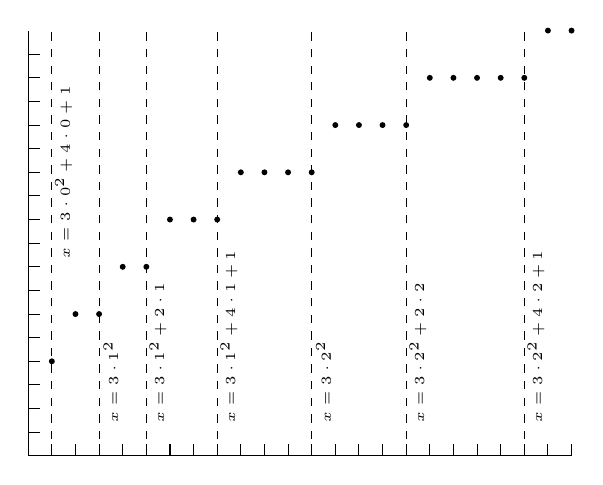
\begin{tikzpicture}[scale=.3]
\draw(0,0)--(23,0);
\draw(0,0)--(0,18);
   \foreach \M in {1,...,23}
   {\draw[fill=black] ({\M},{2*ceil(sqrt(3*\M))}) circle(.1);
   \draw({\M},0)--({\M},.5);}
   \foreach \M in {1,...,17}
   {\draw(0,{\M})--(.5,{\M});}
   \foreach \K in {1,2}
   {
   \draw[dashed] (3*\K*\K,0)--(3*\K*\K,18);
   \node[rotate=90,right] at (3*\K*\K+.5,1) {\tiny{$x=3\cdot\K^2$}};
   \draw[dashed] (3*\K*\K+2*\K,0)--(3*\K*\K+2*\K,18);
   \node[rotate=90,right] at (3*\K*\K+2*\K+.5,1) {\tiny{$x=3\cdot\K^2+2\cdot\K$}};
   \draw[dashed] (3*\K*\K+4*\K+1,0)--(3*\K*\K+4*\K+1,18);
   \node[rotate=90,right] at (3*\K*\K+4*\K+1+.5,1) {\tiny{$x=3\cdot\K^2+4\cdot\K+1$}};
   }
   \draw[dashed] (1,0)--(1,18);
   \node[rotate=90] at (1+.5,12) {\tiny{$x=3\cdot0^2+4\cdot0+1$}};
   
\end{tikzpicture}
\caption{$y=2\ceil{\sqrt{3M}}$, with vertical lines where $J_g(x)>0$.}\label{fig:graph}
\end{figure}

Verifying this, $J_f(M)\neq 0$ if and only if there is a perfect square in the interval $[3M,3(M+1))$.  Thus we have three cases, either $3M\le (3k)^2<3(M+1)$, $3M\le (3k+1)^2<3(M+1)$, or $3M\le (3k+2)^2<3(M+1)$, 
In each case $M=\floor{\sfrac{9k^2}{3}} = 3k^2$, 
$M=\floor{\sfrac{(3k+1)^2}{3}}=3k^2+2k$, 
or $M=\floor{\sfrac{(3k+2)^2}{3}} =3k^2+4k+1$.  This agrees with $J_g(M)$.  An induction with base case $M=3k^2$ completes the proof.\end{proof}

\end{document}
